\documentclass[12pt, letter]{exam}
\usepackage[utf8]{inputenc}
\usepackage[T1]{fontenc}
\usepackage[spanish]{babel}
\usepackage{amsmath}
\usepackage{amsthm}
\usepackage{physics}
\usepackage{tikz}
\usepackage{float}
\usepackage{siunitx}
\usepackage{multicol}
\usepackage[left=2.00cm, right=2.00cm, top=2.00cm, 
     bottom=2.00cm]{geometry}

\renewcommand{\questionlabel}{\thequestion)}
\decimalpoint

\begin{document}

\textbf{Física}.
\begin{questions}
     \question Escribe el estado correspondiente de las partículas que se muestran a continuación:
     \begin{figure}[h]
        \centering
        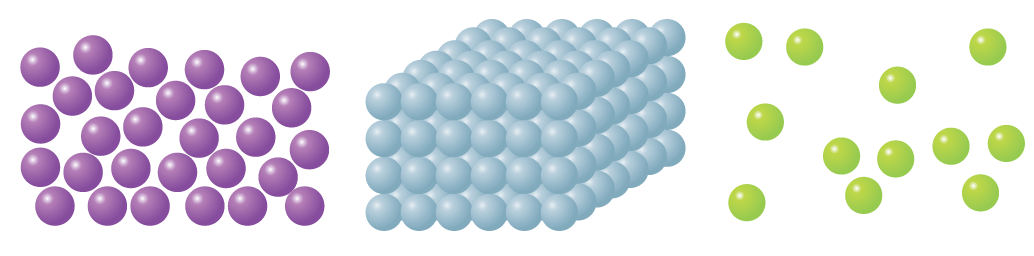
\includegraphics[scale=0.5]{Imagenes/Fisica_01.png}
     \end{figure}
     \begin{choices}
         \choice metal, gas, líquido.
         \choice solido, líquido, gas.
         \choice líquido, sólido, gas.
         \choice gel, gas, agua.
     \end{choices}
\end{questions}
\end{document}